\chapter{系统理论设计和仿真}

本章利用前文描述的基础知识,对基于压缩感知的太阳能组件缺陷检测系统进行理论
设计和数值仿真。首先设计压缩感知系统的核心——测量矩阵 $\Phi$ ,之后以小波域
的 $\ell_1$ 范数优化(Lasso 回归)和空间域的全变分优化方法为例进行数值仿真
实验,以验证采用压缩感知方法检测太阳能组件缺陷的可行性。

\section{感知系统理论设计}

目前的压缩感知理论框架要求线性测量,非线性的稀疏恢复理论尚未成型。根据式
\ref{eqn:LightCurrent} 知道,光电流与面积 $A$ ,以及光通量 $L$ 成正比。
这说明,我们可以采用不同强度的光照射太阳能电池板感光面的各个不同位置,
总的光电流就是各个位置产生的光电流之和:
\begin{equation}
I_L = \sum_i I_i = \sum_i (W_i K_i)  L_i(q_e \cdot \delta A)
\end{equation}
这里 $\delta A$ 是小面积元的大小,而 $(W_i K_i)$ 衡量了位置 $i$ 的光电
转化效率。这个式子就相当于光电转化效率和 $L_i$ 的内积。进行多次测量,每次
采用一组不同的 $L_i$ 。于是, $L_i$ 就相当于测量矩阵 $H$ 中的行,
$I_L$ 就是 $y$ 中的一个采样点。

注意到矩阵中的每一行相当于一组光通量,为简单起见,采用 Bernoulli 矩阵作为
测量矩阵 $H$ 。由于 Bernoulli 矩阵中各个元素相互独立,服从两点($0-1$)
分布,即使光电流与光通量并不严格线性,也不会导致无法恢复。

我们试用两种恢复算法对 $x$ 进行恢复。第一种方法是直接采用全变分最小化方法
(求解问题 \ref{prob:TVopt})恢复 $x$:
\begin{equation}
\hat x = \mathop{\arg\min}_{x'} TV(x') \quad s.t. \quad
\|Hx' - y\|_2 \leq \epsilon
\end{equation}

另一方面,考虑到某些缺陷的边界并不是非常尖锐,采用全变分最小化可能效果
不佳,尝试使用小波基 $\Psi$ 展示 $x$ 的稀疏性:
\begin{equation}
y = Hx = H\Psi a
\end{equation}
定义 $\Phi = H\Psi$,通过 Lasso 回归(求解问题 \ref{prob:Lasso})恢复
稀疏表示 $a$,进而恢复 $x$:
\begin{equation}
\hat x = \Psi \hat a = \Psi \mathop{\arg\min}_{a'} \|a'\|_1 \quad s.t.
\quad \|\Phi a - y\|_2 \leq \epsilon
\end{equation}
注意到根据定理 \ref{th:RandomRIP},当 $H$ 的行数 $M$ 足够大时,矩阵 $\Phi$
以约束等距常数 $\delta_{2K} < 1/3$ 满足 $2K$ 阶 RIP。又根据定理
\ref{th:l1recovery} ,Lasso 回归能够以有限误差重构稀疏表示 $a$。

下面我们将对这两种算法进行数值仿真,以比较它们的优劣。

\section{数值仿真结果}

\subsection{测试用例设计}

为了测试恢复算法的性能,需要设计一些具有代表性的测试用例。这里我们不深究
太阳能组件缺陷的产生原因,仅仅考虑缺陷的形态学特性。缺陷大致可以分为
坏点、裂纹和坏块,图 \ref{fig:testdata} 中的测试用例涵盖了这三种缺陷,
以及栅状电极的影响。

\begin{figure}
\centering
\begin{subfigure}[t]{1in}
	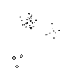
\includegraphics{Figure/testdata/0d.png}
	\caption{坏点}
	\label{fig:testdata:0d}
\end{subfigure}
\begin{subfigure}[t]{1in}
	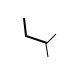
\includegraphics{Figure/testdata/1d.png}
	\caption{裂纹}
	\label{fig:testdata:1d}
\end{subfigure}
\begin{subfigure}[t]{1in}
	
\includegraphics{Figure/testdata/2dsharp.png}
	\caption{边缘清晰的坏块}
\end{subfigure}
\begin{subfigure}[t]{1in}
	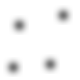
\includegraphics{Figure/testdata/2dsmooth.png}
	\caption{边缘模糊的坏块}
\end{subfigure}
\begin{subfigure}[t]{1in}
	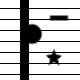
\includegraphics{Figure/testdata/2dsharp_finger.png}
	\caption{坏块与栅状电极}
\end{subfigure}
\caption{测试用例}
\label{fig:testdata}
\end{figure}

\subsection{全变分最小化重建的仿真结果}

本文中,所有全变分最小化重建均使用 Li 编写的 \verb|TVAL3| 软件包完成。
该软件包
采用增广拉格朗日乘子法和交替方向算法求解全变分最小化重建问题,是一款非常
优秀的全变分最小化求解器。关于该软件包的设计思路和实现细节,参见文献
\cite{TVAL3CBLMaster} \cite{TVAL3CBLPhD}。

\paragraph{对坏点的重建结果} 图 \ref{fig:TV0d} 给出了图 
\ref{fig:testdata:0d} 以 $M$ 行 Bernoulli 矩阵作为测量矩阵采样后的 TV 最小
化恢复结果,采样结果中加入 $10\%$ 的高斯白噪声。

\begin{figure}
\centering
\begin{subfigure}[t]{1in}
	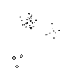
\includegraphics{Figure/testdata/0d.png}
	\caption{原始数据}
\end{subfigure}
\begin{subfigure}[t]{1in}
	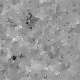
\includegraphics{Figure/TV/0d10.png}
	\caption{$M = 0.1 N$,相对误差 $43.97\%$}
\end{subfigure}
\begin{subfigure}[t]{1in}
	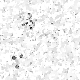
\includegraphics{Figure/TV/0d30.png}
	\caption{$M = 0.3 N$,相对误差 $12.48\%$}
\end{subfigure}
\begin{subfigure}[t]{1in}
	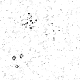
\includegraphics{Figure/TV/0d50.png}
	\caption{$M = 0.5 N$,相对误差 $8.39\%$}
\end{subfigure}
\begin{subfigure}[t]{1in}
	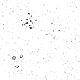
\includegraphics{Figure/TV/0d70.png}
	\caption{$M = 0.7 N$,相对误差 $9.34\%$}
\end{subfigure}
\caption{坏点的全变分最小化重建结果}
\label{fig:TV0d}
\end{figure}

可见, $M = 0.1 N$ 时重建完全失败,这是由于 $M$ 太小,不满足定理
\ref{th:RandomRIP} 的要求,导致矩阵 $H$ 丧失 RIP 性质。然而,重建
效果也并非随着 $M$ 的增加而单调增加,这是由于随着矩阵规模的增加,
约束条件 $\|Hx' - y\| \leq \epsilon$ 对 $x'$ 来说更加严格,导致
优化问题的自由度降低,全变分最小化的去噪作用未能充分发挥,从而
使得噪声 $z$ 对结果产生较大影响。

\paragraph{对裂纹的重建结果} 图 \ref{fig:TV1d} 给出测试数据
\ref{fig:testdata:1d} 的重建结果,测量矩阵 $H$ 和加性噪声 $z$
同上。

\begin{figure}
\centering
\begin{subfigure}[t]{1in}
	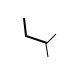
\includegraphics{Figure/testdata/1d.png}
	\caption{原始数据}
\end{subfigure}
\begin{subfigure}[t]{1in}
	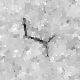
\includegraphics{Figure/TV/1d10.png}
	\caption{$M = 0.1 N$,相对误差 $22.01\%$}
\end{subfigure}
\begin{subfigure}[t]{1in}
	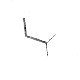
\includegraphics{Figure/TV/1d30.png}
	\caption{$M = 0.3 N$,相对误差 $19.56\%$}
\end{subfigure}
\begin{subfigure}[t]{1in}
	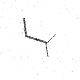
\includegraphics{Figure/TV/1d50.png}
	\caption{$M = 0.5 N$,相对误差 $24.63\%$}
\end{subfigure}
\begin{subfigure}[t]{1in}
	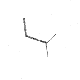
\includegraphics{Figure/TV/1d70.png}
	\caption{$M = 0.7 N$,相对误差 $39.38\%$}
\end{subfigure}
\caption{裂纹的全变分最小化重建结果}
\label{fig:TV1d}
\end{figure}

除了 $M = 0.1N$ 时重建结果很差外,其他三次重建都较好地恢复了
图像中的裂纹。然而,可以注意到裂纹出现较为明显的锯齿,这是由于
全变分最小化会促进图像梯度的稀疏性,导致图像出现类似阶梯函数的
特性。

\paragraph{对边界清晰的坏块重建结果} 见图 \ref{fig:TV2dsharp}。
可以看出,全变分最小化对边界稀疏的图像重建效果很好,甚至只要
$10\%$ 的采样即可几乎完美地恢复出图像中的三个坏块。

\begin{figure}
\centering
\begin{subfigure}[t]{1in}
	
\includegraphics{Figure/testdata/2dsharp.png}
	\caption{原始数据}
\end{subfigure}
\begin{subfigure}[t]{1in}
	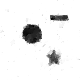
\includegraphics{Figure/TV/2dsharp10.png}
	\caption{$M = 0.1 N$,相对误差 $7.98\%$}
\end{subfigure}
\begin{subfigure}[t]{1in}
	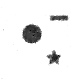
\includegraphics{Figure/TV/2dsharp30.png}
	\caption{$M = 0.3 N$,相对误差 $23.88\%$}
\end{subfigure}
\begin{subfigure}[t]{1in}
	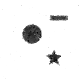
\includegraphics{Figure/TV/2dsharp50.png}
	\caption{$M = 0.5 N$,相对误差 $35.97\%$}
\end{subfigure}
\begin{subfigure}[t]{1in}
	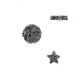
\includegraphics{Figure/TV/2dsharp70.png}
	\caption{$M = 0.7 N$,相对误差 $38.66\%$}
\end{subfigure}
\caption{边界清晰坏块的全变分最小化重建结果}
\label{fig:TV2dsharp}
\end{figure}

\paragraph{对边界模糊的坏块重建结果}

\paragraph{对栅状电极的重建结果}
